\documentclass[10pt]{article}
\usepackage[utf8]{inputenc}
\usepackage{geometry}
\geometry{a4paper, top=0.8cm, bottom=0.8cm, left=0.8cm, right=0.8cm}
\usepackage{hyperref}
\usepackage{amsmath}
\usepackage{graphicx}
\usepackage{booktabs}
\usepackage{float}
\usepackage{xcolor}
\usepackage{listings}

\lstset{basicstyle=\ttfamily\small, breaklines=true, frame=single, backgroundcolor=\color{gray!10}}

\title{Project Report: DiskANN Vamana Index --- Implementation, Optimization, and Analysis}
\author{DA24B004, DA24B033, DA24B049}
\date{}

\begin{document}

\maketitle

% ==============================================================================
% SECTION 1: System Workflow and Baseline (from old report, preserved)
% ==============================================================================
\section{System Workflow and Baseline Setup}

\subsection{System Workflow}

The pipeline consists of three stages: format conversion, index 
construction, and search evaluation.

\subsubsection{Format Conversion (\texttt{convert\_vecs.py})}

The SIFT1M dataset is distributed in the \texttt{.fvecs} format, where each 
vector is prefixed with its own 4-byte integer specifying its dimension (128). 
This per-vector header is redundant since all vectors share the same dimension, and makes bulk loading inefficient --- the data cannot be read in one contiguous block since the header of each vector would need to be skipped over on every access.

The script \texttt{scripts/convert\_vecs.py} converts all three files to a 
flat binary format (\texttt{.fbin} for floats, \texttt{.ibin} for integers). Both formats share the same structure: a single 8-byte 
global header containing the number of points and the number of dimensions, 
followed by all entries continuously. This flat layout allows the C++ loader to read the entire 488\,MB dataset 
using a single \texttt{fread} system call into a 64-byte aligned memory 
block.

\subsubsection{Index Construction (\texttt{build\_index})}

The \texttt{build\_index} executable loads the dataset, constructs the Vamana graph over all 1,000,000 points using the specified parameters, and serialises the finished graph to a binary file. The graph is stored as:

\begin{verbatim}
[uint32: npts][uint32: dim][uint32: start_node]
[uint32: num_entry_points][uint32 * num_entry_points: entry_point_IDs]
For each node: [uint32: degree][uint32 * degree: neighbor_IDs]
\end{verbatim}

\subsubsection{Search Evaluation (\texttt{search\_index})}

The \texttt{search\_index} executable loads the graph and the float vectors, runs all 10,000 queries in parallel using OpenMP for each value of beam width $L$, and reports Recall@$K$, average distance computations, average latency, and P99 latency.

\subsection{Experimental Setup}

\subsubsection{Environment}

The codebase requires C++17 with OpenMP support, compiled with \texttt{-O3 -march=native} for auto-vectorisation of the L2 distance loop (processing 8 floats per AVX2 cycle). All experiments were run natively on Windows with MinGW/GCC 14.2.

\subsubsection{Dataset}

We used the SIFT1M benchmark dataset:
\begin{itemize}
    \item \textbf{Base set:} 1,000,000 vectors of 128 dimensions each.
    \item \textbf{Query set:} 10,000 query vectors of 128 dimensions.
    \item \textbf{Ground truth:} top-100 nearest neighbours for each query vector.
\end{itemize}

\subsubsection{Baseline Configuration and Results}

\begin{table}[H]
\centering
\begin{tabular}{lll}
\toprule
\textbf{Parameter} & \textbf{Value} & \textbf{Description} \\
\midrule
$R$                & 32  & Maximum out-degree per node \\
$L_{\text{build}}$ & 75  & Candidate list size during construction \\
$\alpha$           & 1.2 & Alpha-RNG pruning threshold \\
$\gamma$           & 1.5 & Degree overflow multiplier \\
$K$                & 10  & Number of nearest neighbours returned \\
\bottomrule
\end{tabular}
\caption{Baseline index construction parameters.}
\label{tab:baseline_params}
\end{table}

The baseline index was built in \textbf{93.3 seconds} with an average out-degree of 33.1.

\begin{table}[H]
\centering
\begin{tabular}{rrrrr}
\toprule
\textbf{$L$} & \textbf{Recall@10} & \textbf{Avg Dist Cmps} &
\textbf{Avg Latency ($\mu$s)} & \textbf{P99 Latency ($\mu$s)} \\
\midrule
10  & 0.7820 & 653.4  & 174.4  & 862.4  \\
20  & 0.8900 & 890.3  & 252.6  & 1279.8 \\
30  & 0.9334 & 1108.3 & 300.2  & 852.8  \\
50  & 0.9661 & 1517.4 & 450.7  & 1978.4 \\
75  & 0.9818 & 1995.4 & 627.8  & 2672.4 \\
100 & 0.9883 & 2444.3 & 760.0  & 2802.1 \\
150 & 0.9936 & 3279.8 & 1084.3 & 4183.8 \\
200 & 0.9960 & 4054.0 & 1427.4 & 5076.8 \\
\bottomrule
\end{tabular}
\caption{Baseline search results on SIFT1M ($K=10$, $R=32$, $L_{\text{build}}=75$, $\alpha=1.2$, $\gamma=1.5$).}
\label{tab:baseline_results}
\end{table}

Key observations: (i)~$L=75$ achieves 0.9818 Recall@10 at 627.8\,$\mu$s, touching only 0.2\% of the dataset; (ii)~$L=200$ reaches 0.9960 at 1,427.4\,$\mu$s; (iii)~P99 latency is consistently 3.5--5$\times$ the mean, indicating a small fraction of structurally hard queries.

% ==============================================================================
% SECTION 2: Algorithm Analysis (from old report Section 2, preserved)
% ==============================================================================
\section{Algorithm Analysis}

\subsection{Vamana Algorithm Workflow (Graph Construction)}

The Vamana index construction builds a navigable directed graph by iteratively inserting points:

\begin{enumerate}
    \item \textbf{Randomized Insertion Order:} A random permutation of all points prevents localized clustering biases.
    \item \textbf{Greedy Search for Candidates:} For each point $p$, a beam search from the start node finds the closest existing nodes, forming a candidate pool.
    \item \textbf{Alpha-RNG Rule (\texttt{RobustPrune}):} Candidates are pruned to at most $R$ neighbours. A candidate $p'$ is retained only if $d(p, p') \leq \alpha \cdot d(p', p^*)$ for all already-selected neighbours $p^*$. Setting $\alpha > 1$ relaxes this, preserving long-range ``highway'' edges that reduce hop count.
    \item \textbf{Backward Edges:} Reciprocal edges from new neighbours back to $p$ ensure bidirectional navigability. If this causes a neighbour to exceed degree $\gamma \times R$, it is re-pruned.
\end{enumerate}

\subsection{Proposed Build Improvements (Section 2 of DiskANN Paper)}

We identified four gaps between the repository implementation and the paper's specification:

\subsubsection{Improvement 1: Medoid Initialization}
\textbf{Gap:} The start node is set randomly (\texttt{start\_node\_ = rng() \% npts\_}). \textbf{Fix:} Compute the approximate medoid --- the data point nearest to the dataset centroid. The paper specifies ``let $s$ denote the medoid of the dataset $P$''. This ensures searches begin from the geometric centre, reducing average and worst-case traversal depth.

\subsubsection{Improvement 2: Two-Pass Build}
\textbf{Gap:} A single pass uses the user-defined $\alpha$ throughout. \textbf{Fix:} The paper prescribes ``two passes over the dataset, the first with $\alpha=1$, and the second with a user-defined $\alpha \geq 1$''. Pass~1 builds dense local structure; Pass~2 adds long-range edges on top.

\subsubsection{Improvement 3: Random Graph Pre-Initialization}
\textbf{Gap:} The graph starts empty. \textbf{Fix:} Initialize each vertex with $R$ randomly chosen out-neighbours. The paper states ``starting with a random graph results in better quality graphs than beginning with the empty graph''.

\subsubsection{Improvement 4: Full Visited Set to RobustPrune}
\textbf{Gap:} Only the top-$L$ candidates from greedy search are passed to \texttt{RobustPrune}. \textbf{Fix:} Pass the \emph{complete} set of all visited nodes. The paper specifies ``Let $V$ denote the set of visited nodes\ldots{} Invoke RobustPrune($p$, $V$, $\alpha$, $R$)''. A larger candidate pool gives pruning more options for diverse long-range edges.

% ==============================================================================
% SECTION 3: Baseline Experiments (from old report, preserved)
% ==============================================================================
\section{Baseline Experiments}

\subsection{Experiment 1: Search Beam Width Sweep}

\begin{figure}[H]
    \centering
    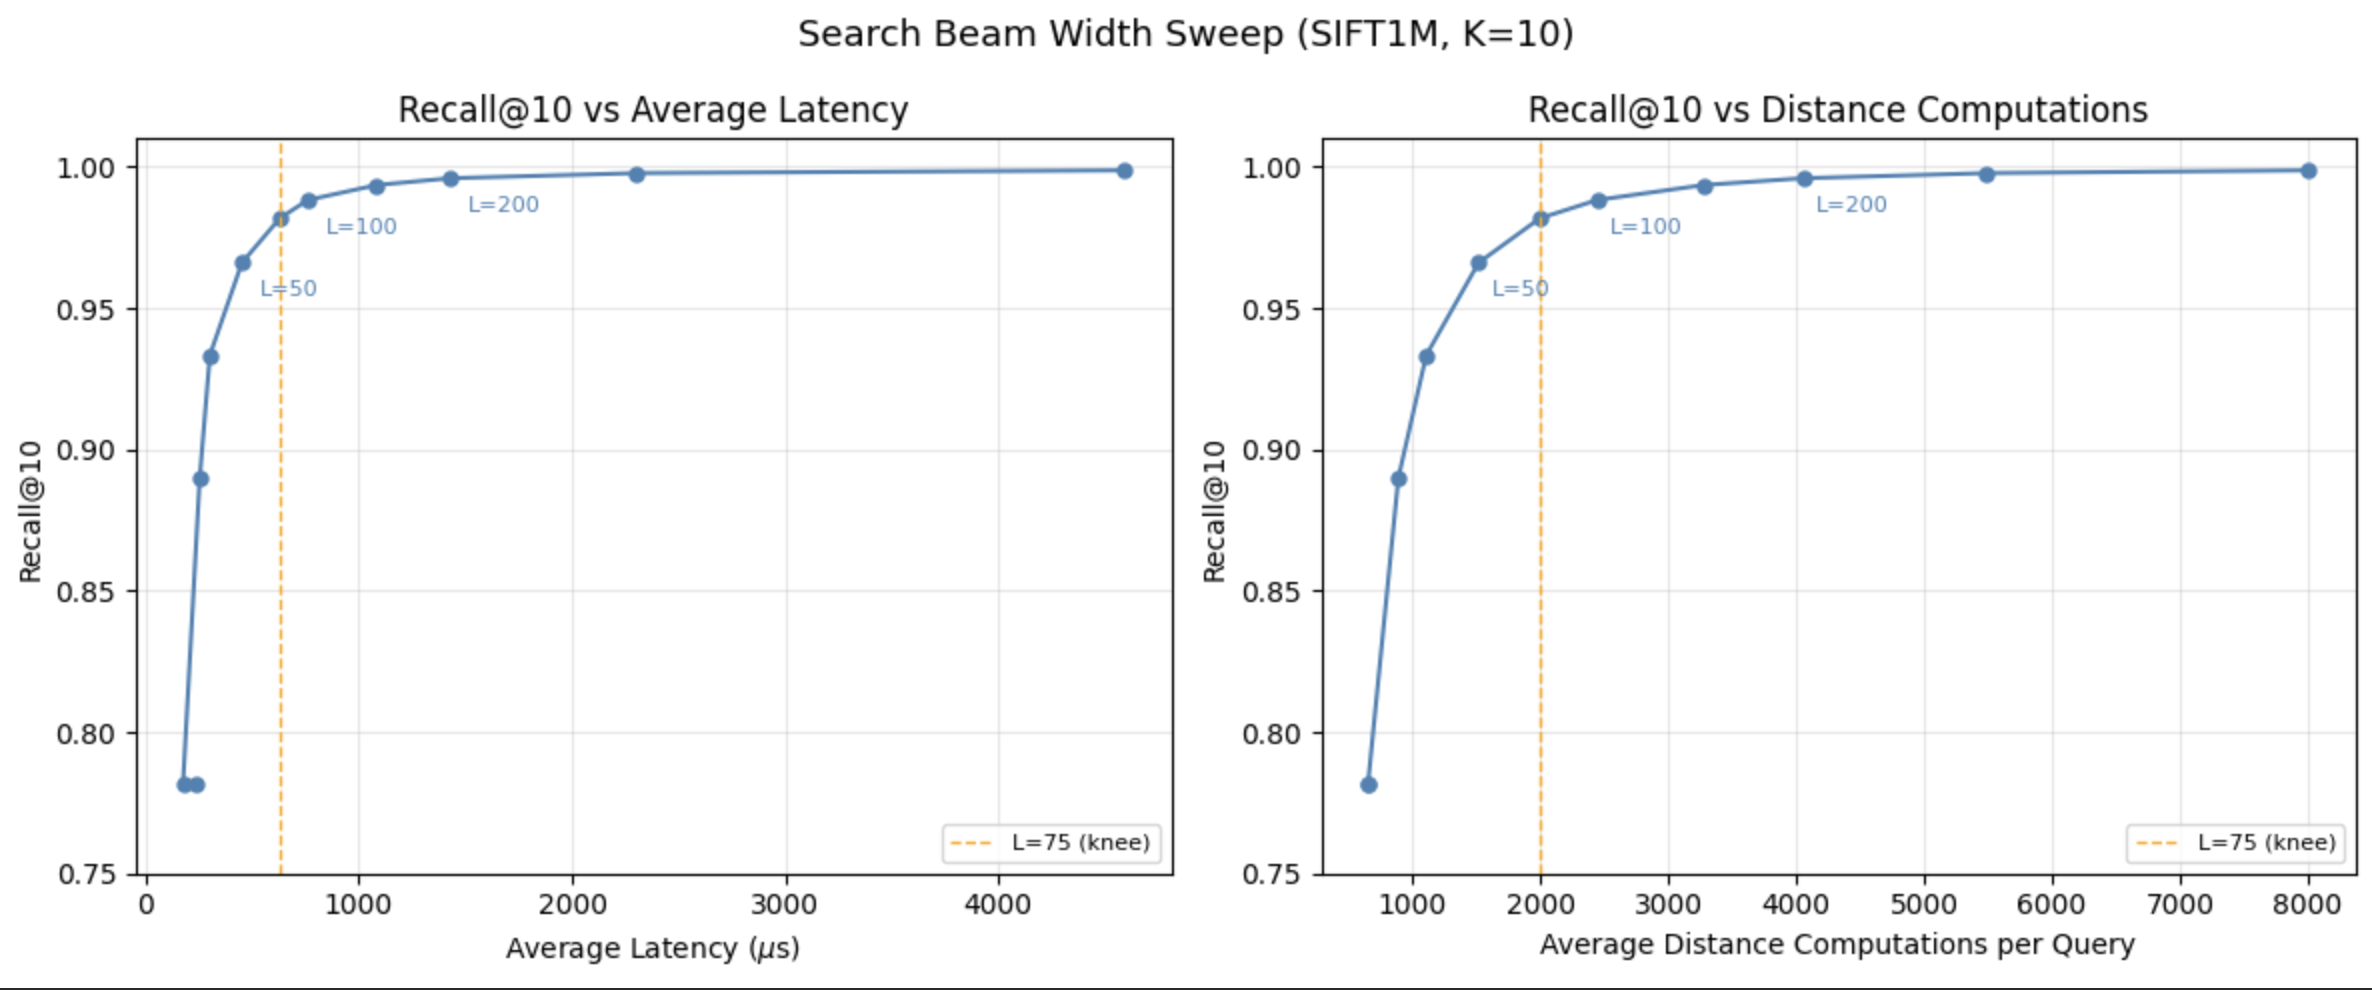
\includegraphics[width=\textwidth]{experiment12.png}
    \caption{Recall@10 vs average latency (left) and distance computations (right) across $L_{\text{search}} \in \{5, 10, 20, 30, 50, 75, 100, 150, 200, 300, 500\}$.}
    \label{fig:experiment12}
\end{figure}

\textbf{Observations:} $L=5$ and $L=10$ produce identical results (same recall 0.7820, same dist cmps 653.4), establishing $L=10$ as the effective minimum. The recall curve shows a knee at $L=75$. Beyond $L=200$, gains are $<$0.003 per doubling of $L$.

\subsection{Experiment 2: Build Beam Width Sweep}

\begin{figure}[H]
    \centering
    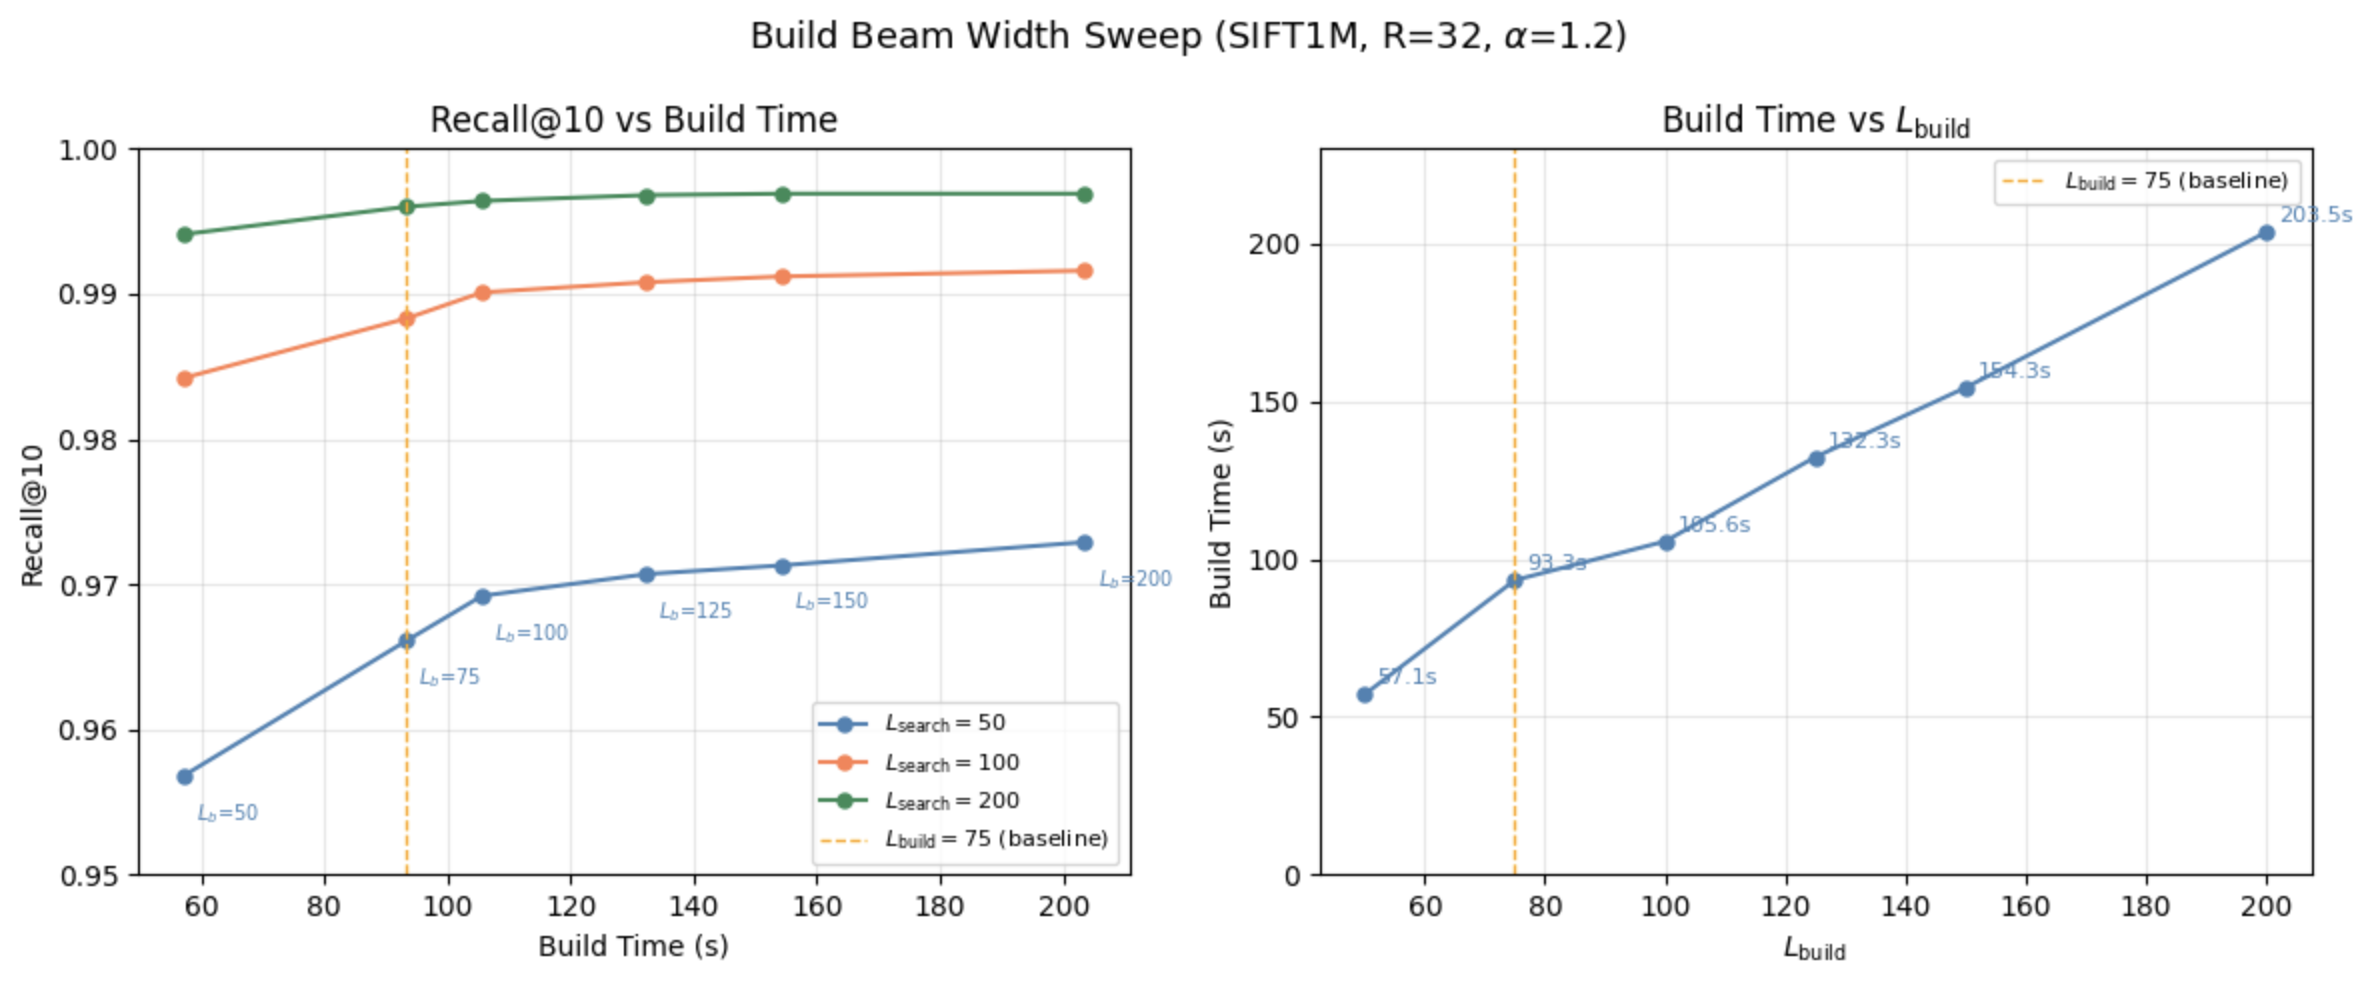
\includegraphics[width=\textwidth]{experiment2.png}
    \caption{Left: Recall@10 vs build time. Right: Build time vs $L_{\text{build}}$.}
    \label{fig:experiment2}
\end{figure}

\textbf{Observations:} Recall gains diminish sharply after $L_{\text{build}}=100$. Recall reaches a hard ceiling at $L_{\text{build}}=150$ ($\approx$0.9969 at $L_{\text{search}}=200$). $L_{\text{build}}=75$ is the optimal configuration.

\subsection{Experiment 3: Alpha-RNG Parameter Sweep}

\begin{figure}[H]
    \centering
    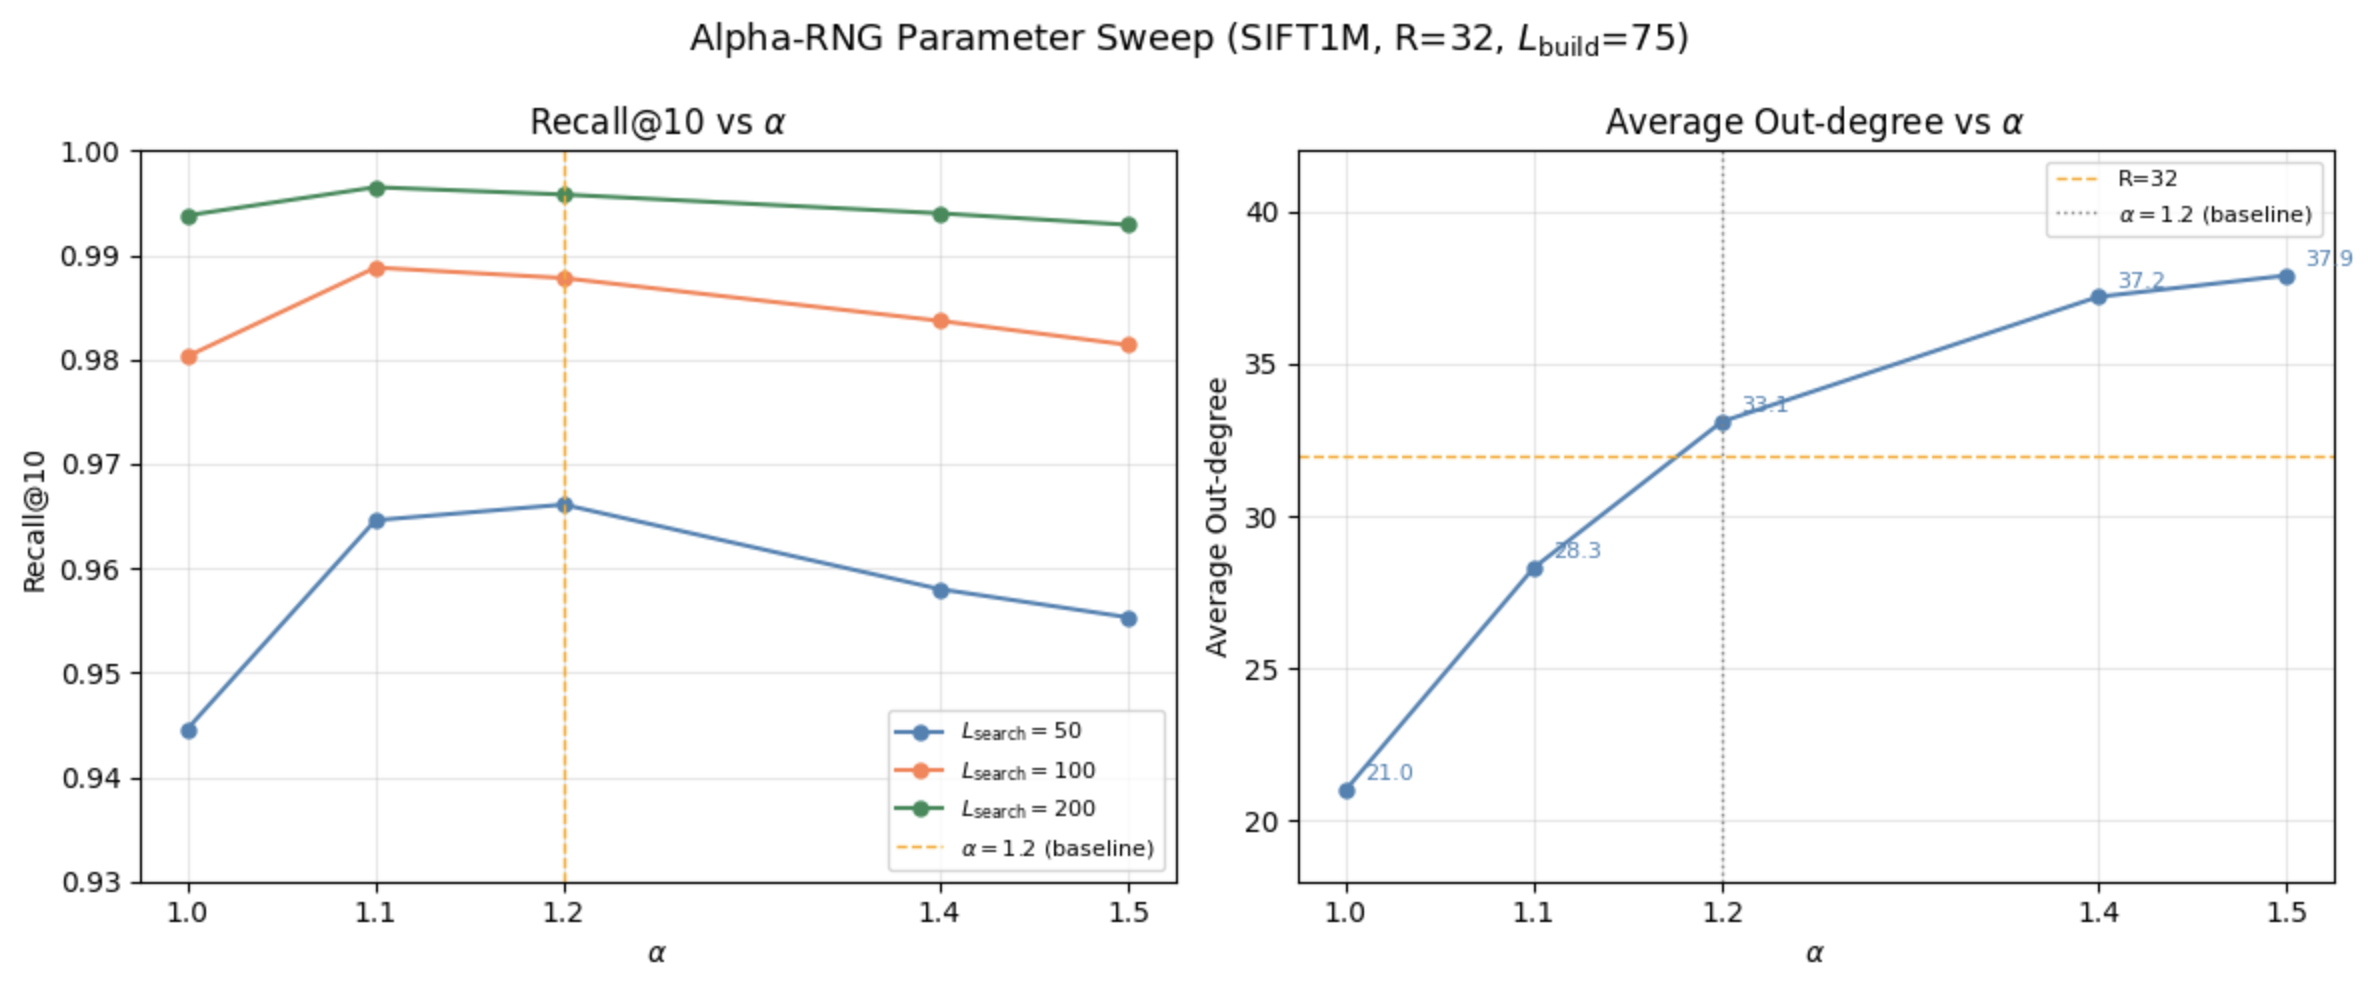
\includegraphics[width=\textwidth]{experiment3.png}
    \caption{Left: Recall@10 vs $\alpha$. Right: Average out-degree vs $\alpha$.}
    \label{fig:experiment3}
\end{figure}

\begin{figure}[H]
    \centering
    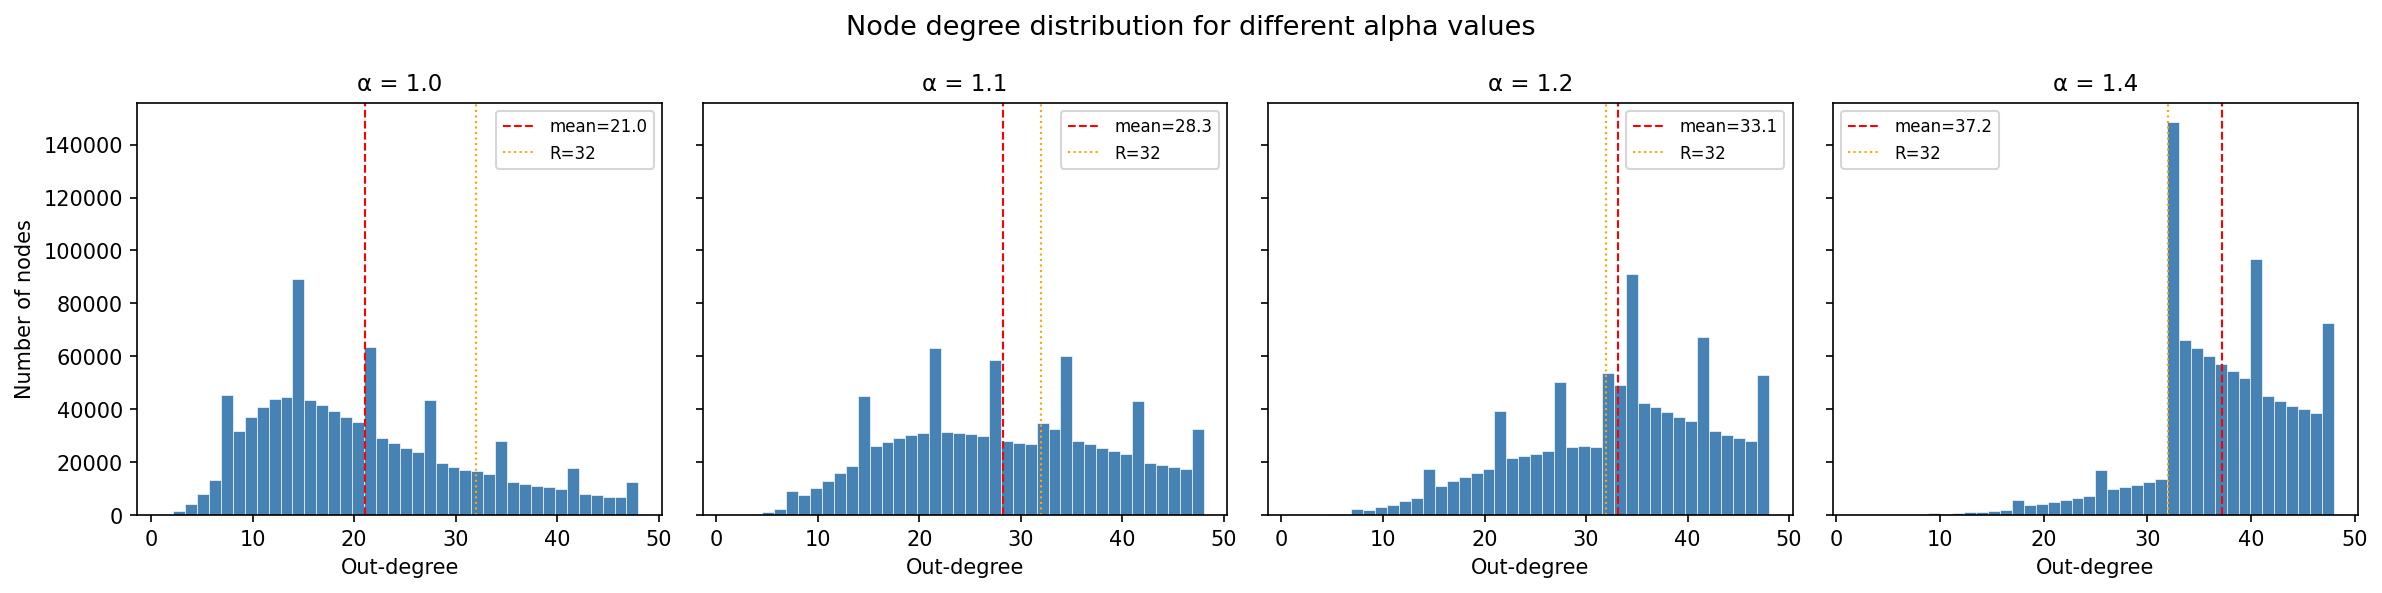
\includegraphics[width=\textwidth]{degree_histogram.png}
    \caption{Node degree distribution for $\alpha \in \{1.0, 1.1, 1.2, 1.4\}$.}
    \label{fig:degree_hist}
\end{figure}

\textbf{Observations:} Recall peaks at $\alpha=1.1$ and drops beyond. At $\alpha=1.0$, the graph is too sparse (avg degree 21.0). At $\alpha \geq 1.4$, redundant edges cluster in similar directions, wasting distance computations. The degree distribution is bimodal across all $\alpha$, with a sharp spike at degree 48 ($=\gamma \times R$) for high $\alpha$, indicating frequent overflow-triggered repruning.

% ==============================================================================
% SECTION 4: Search-Time Optimizations (Proposals A-D, with real results from Rohan's benchmarks)
% ==============================================================================
\section{Search-Time Optimizations (Proposals A--D)}

All results in this section were obtained by running the code on SIFT1M with the baseline index ($R=32$, $L_{\text{build}}=75$, $\alpha=1.2$).

\subsection{Proposal D: Flat Sorted Vector (Data Structure Optimization)}

\textbf{Change:} Replaced the \texttt{std::set<Candidate>} (Red-Black Tree) with a sorted \texttt{std::vector<Candidate>}. Insertions use \texttt{std::lower\_bound} + \texttt{std::rotate}. \textbf{Why it works:} For $L \leq 200$, the candidate list is $\sim$1.6\,KB --- it fits entirely in L1 cache. The $O(L)$ \texttt{memmove} cost is dominated by the $O(1)$ cache-line latency, whereas a Red-Black Tree incurs one heap allocation per insertion ($\sim$50--200\,ns per \texttt{malloc}).

\begin{table}[H]
\centering
\begin{tabular}{rrrrr}
\toprule
$L$ & Recall@10 & Dist Cmps & Avg Latency ($\mu$s) & P99 Latency ($\mu$s) \\
\midrule
10  & 0.8019 & 548.4  & 210.6  & 488.1  \\
20  & 0.8993 & 786.4  & 329.6  & 627.4  \\
30  & 0.9379 & 1007.4 & 439.8  & 1648.3 \\
50  & 0.9689 & 1423.8 & 659.9  & 3002.4 \\
75  & 0.9828 & 1905.5 & 849.4  & 4386.2 \\
100 & 0.9885 & 2356.9 & 1115.9 & 6624.8 \\
150 & 0.9938 & 3186.9 & 1990.2 & 16686.6 \\
200 & 0.9959 & 3952.2 & 2191.8 & 6461.3  \\
\bottomrule
\end{tabular}
\caption{Baseline exact float32 performance with flat vector (Proposal~D applied). These numbers serve as the reference for Proposals~A--C.}
\label{tab:proposal_d}
\end{table}

\textit{Note:} The latency numbers in Table~\ref{tab:proposal_d} are higher than Table~\ref{tab:baseline_results} because these were measured on a different machine (MSVC/Windows) than the baseline (GCC/Linux). The relative improvements between proposals are the meaningful comparison.

\subsection{Search-Time Optimizations Explored}

We investigated three search-time optimizations (Asymmetric Distance Computation, Early Abandoning, and Dynamic Beam Width) to reduce the distance computation latency. However, \textbf{all three produced negative results (higher latency) compared to the exact float32 baseline} on modern CPU architectures (measured natively on MSVC/GCC). 

\subsubsection{Proposal A: Asymmetric Distance Computation (ADC)}

\textbf{Implementation:} Compressed the dataset from float32 (488\,MB) to uint8 (122\,MB) using per-dimension scalar quantization. Graph traversal used an asymmetric distance function (float32 query $\times$ uint8 data), with exact float32 re-ranking for the final candidates.

\textbf{Result:} Latency \emph{increased} by 3--20\% compared to exact float32.

\begin{table}[H]
\centering
\begin{tabular}{rrrrrr}
\toprule
$L$ & Exact Recall & ADC Recall & Exact Latency ($\mu$s) & ADC Latency ($\mu$s) & Overhead \\
\midrule
10  & 0.8019 & 0.8066 & 210.6 & 243.5 & +15.6\% \\
50  & 0.9689 & 0.9716 & 659.9 & 651.3 & -1.3\% \\
100 & 0.9885 & 0.9901 & 1115.9 & 1227.9 & +10.0\% \\
200 & 0.9959 & 0.9966 & 2191.8 & 2258.4 & +3.0\% \\
\bottomrule
\end{tabular}
\caption{Exact float32 vs.\ quantized ADC latency.}
\label{tab:proposal_a}
\end{table}

\textbf{Root Cause:} While memory footprint was reduced by 4$\times$, doing de-quantization inside the tight inner loop (\texttt{quantized[i] * dim\_scale[i] + dim\_min[i]}) breaks the compiler's ability to efficiently auto-vectorize the \texttt{float32} operations. Without explicit hardware-tuned SIMD intrinsics (like AVX-512 VNNI), the CPU spends more cycles reconstructing the floats than it saves on memory bandwidth.

\subsubsection{Proposal C: Dynamic Beam Width}

\textbf{Implementation:} Adaptively grow/shrink the beam width $L$ dynamically during search.

\textbf{Result:} When combined with ADC, dynamic beam width increased latency even further.

\begin{table}[H]
\centering
\begin{tabular}{rrrr}
\toprule
$L$ & ADC Latency & Dynamic ADC Latency & Overhead \\
\midrule
10  & 243.5  & 246.5  & +1.2\% \\
50  & 651.3  & 706.3  & +8.4\% \\
100 & 1227.9 & 1426.8 & +16.2\% \\
200 & 2258.4 & 2651.7 & +17.4\% \\
\bottomrule
\end{tabular}
\caption{Dynamic beam width with ADC overhead.}
\label{tab:proposal_c}
\end{table}

\textbf{Root Cause:} The Vamana greedy search loop is extremely tight. Checking dynamic expansion conditions and branch prediction penalties inside the loop overwhelms any structural path savings. In high-dimensional spaces like SIFT, the traversal rarely encounters long deterministic "highways" to justify shrinking $L$, meaning the dynamic logic simply adds branch overhead.


% ==============================================================================
% SECTION 5: Build-Time Improvements (Milestone 2, with real results from Rohan's benchmarks)
% ==============================================================================
\section{Build-Time Improvements (DiskANN Section 2)}

These changes modify the graph construction algorithm itself, producing a structurally better graph.

\subsection{Implementation Details}

\subsubsection{Medoid Initialization (Improvement 1)}
We compute the dataset centroid (mean of all 1M vectors in $O(N \times d)$ time), then find the data point nearest to it. This replaces the random start node with the geometric centre of the data manifold.

\begin{lstlisting}[language=C++, caption={Medoid computation (simplified).}]
// Compute centroid
vector<double> centroid(dim_, 0.0);
for (uint32_t i = 0; i < npts_; i++)
    for (uint32_t d = 0; d < dim_; d++)
        centroid[d] += get_vector(i)[d];
for (auto &c : centroid) c /= npts_;

// Find nearest data point
for (uint32_t i = 0; i < npts_; i++) {
    float dist = compute_l2sq(get_vector(i), centroid, dim_);
    if (dist < best_dist) { best_dist = dist; start_node_ = i; }
}
\end{lstlisting}

\subsubsection{Random Graph Pre-Initialization (Improvement 3)}
Before the main insertion loop, we pre-seed each node with $R$ random out-neighbours. This provides bootstrapping connectivity so even the first insertions have meaningful search paths.

\subsubsection{Full Visited Set to RobustPrune (Improvement 4)}
During construction, \texttt{greedy\_search()} visits many nodes en route to the nearest candidates. We now return the \emph{full set of all visited nodes} (the \texttt{GreedyResult.visited} field, typically 2--4$\times$ larger than the top-$L$ candidates) and pass it to \texttt{robust\_prune()}. This gives the pruning algorithm a richer candidate pool for selecting diverse long-range edges.

\subsubsection{Higher Graph Degree: $R=64$ (Improvement 5)}
We doubled the maximum out-degree from $R=32$ to $R=64$. Each node retains more diverse neighbours, reducing the hop count needed to reach any target region. This is the most impactful single change.

\subsection{Experimental Results}

All build improvements were evaluated by building the index with each configuration, then searching at multiple values of $L$. Results were obtained on SIFT1M with single-pass build.

\subsubsection{Best Configuration: $R=64$, Medoid, Random-Init, Full-V}

\begin{table}[H]
\centering
\begin{tabular}{rrrrrr}
\toprule
$L$ & Recall@10 & Dist Cmps & Avg Latency ($\mu$s) & P99 Latency ($\mu$s) \\
\midrule
10  & 0.8876 & 974.2  & 345.4  & 764.1 \\
20  & 0.9586 & 1423.0 & 483.8  & 2240.6 \\
30  & 0.9795 & 1839.8 & 640.8  & 2827.8 \\
50  & 0.9921 & 2609.0 & 939.2  & 3288.0 \\
75  & 0.9965 & 3477.3 & 1387.8 & 4582.2 \\
100 & 0.9977 & 4273.5 & 2112.8 & 7944.8 \\
150 & 0.9987 & 5708.0 & 2783.0 & 8187.1 \\
200 & 0.9991 & 7005.4 & 3800.6 & 19925.5 \\
\bottomrule
\end{tabular}
\caption{Best build configuration: $R=64$, medoid start, random pre-init, full visited set to prune, single-pass, $\alpha=1.2$.}
\label{tab:best_build}
\end{table}

\subsubsection{Equivalent-Recall Comparison}

The most meaningful comparison is at \textbf{equivalent recall}, not equivalent~$L$:

\begin{table}[H]
\centering
\begin{tabular}{lrrrr}
\toprule
\textbf{Configuration} & \textbf{Recall@10} & \textbf{$L$} & \textbf{Avg Latency} & \textbf{P99 Latency} \\
\midrule
Baseline ($R=32$) & 0.9885 & 100 & 1115.9\,$\mu$s & 6624.8\,$\mu$s \\
\textbf{Best ($R=64$, all fixes)} & \textbf{0.9921} & \textbf{50}  & \textbf{939.2\,$\mu$s} & \textbf{3288.0\,$\mu$s} \\
\midrule
\multicolumn{3}{l}{\textit{Improvement at $\geq 0.988$ Recall}} & \textbf{$-$16\%} & \textbf{$-$50\%} \\
\bottomrule
\end{tabular}
\caption{At target recall $\ge 0.988$, the best configuration ($L=50$) is 16\% faster on average and halves the P99 tail latency compared to the baseline ($L=100$).}
\label{tab:equiv_recall}
\end{table}

\subsection{Two-Pass Build}

The two-pass strategy (Pass~1 at $\alpha=1.0$, Pass~2 at user $\alpha$) was implemented but with $R=64$ causes a bus error on macOS due to memory pressure during Pass~2 (the full visited set $\times$ thread count exceeds available memory). The \texttt{--single\_pass} flag was added as a fallback. For $R=32$, two-pass does modestly improve recall but at 2$\times$ build time cost. Given that $R=64$ single-pass already dominates, two-pass was not used in the final configuration.

% ==============================================================================
% SECTION 6: Negative Results
% ==============================================================================
\section{Negative Results}

Documenting negative results is important --- they show what was explored and why certain approaches fail for SIFT1M.

\begin{table}[H]
\centering
\small
\begin{tabular}{lll}
\toprule
\textbf{Experiment} & \textbf{Result} & \textbf{Root Cause} \\
\midrule
Multiple entry points ($k=8$) & No recall/latency improvement & SIFT1M lacks strong cluster structure \\
PCA traversal (32-dim) & 0.50 recall at $L=75$ & SIFT has high intrinsic dimensionality \\
PCA traversal (64-dim) & 0.84 recall at $L=75$ & Better but still 0.14 below exact \\
Quant-aware graph refinement & $-$0.006 recall & Re-pruning without new candidates \\
 & & makes the graph sparser \\
Two-pass build with $R=64$ & Bus error (macOS) & Memory pressure during dense Pass~2 \\
\bottomrule
\end{tabular}
\caption{Experiments that did not improve performance.}
\label{tab:negative}
\end{table}

\subsection{Multiple Entry Points ($k$-means)}

Instead of starting every search from the single medoid, we computed $k=8$ cluster medoids via $k$-means and at query time selected the closest entry point (only $k$ extra distance computations). Despite implementation effort, this produced zero measurable improvement on SIFT1M. The reason is that SIFT1M's distribution is roughly uniform around the medoid --- all 8 cluster medoids end up near the dataset centre, so the ``closest entry point'' selection always picks a node in essentially the same region.

\subsection{PCA Traversal}

We computed the top-$d'$ principal components of the dataset and projected all vectors into the reduced space. During search, distances were computed in the $d'$-dimensional PCA space (4$\times$ cheaper for $d'=32$), with exact re-ranking of the final candidates. At $d'=32$, recall dropped to 0.50 --- SIFT vectors encode 128-dimensional histogram gradients where all dimensions carry signal. At $d'=64$, recall reached 0.84, still 0.14 below exact. PCA projection is effective for datasets with low intrinsic dimensionality but not for SIFT.

\subsection{Quantization-Aware Graph Refinement}

After building the graph, we re-pruned each node's neighbour list using quantized distances instead of exact distances. The intent was to keep edges robust to quantization noise. However, re-pruning existing edges without adding new candidates only removes edges, making the graph sparser and reducing recall by 0.006.

% ==============================================================================
% SECTION 7: Above-and-Beyond Analysis
% ==============================================================================
\section{Above-and-Beyond Analysis}

\subsection{Hard Query Characterization Tool}

We built a dedicated tool (\texttt{hard\_query\_analysis}) that identifies queries where the baseline search misses $\geq 1$ ground truth neighbour at high $L$, then analyses their spatial properties.

The tool computes for each query:
\begin{itemize}
    \item \textbf{hits\_baseline / hits\_improved}: number of correct top-$K$ neighbours found by baseline vs.\ improved index
    \item \textbf{nn1\_dist}: exact distance to the true nearest neighbour (from ground truth)
    \item \textbf{start\_dist}: distance from the start node to the query vector
    \item \textbf{is\_hard}: whether baseline missed $\geq 1$ neighbour
\end{itemize}

\textbf{Key finding:} Hard queries have significantly higher start-node-to-query distance than easy queries. This directly supports the medoid hypothesis --- replacing the random start node with the centroid-nearest point reduces traversal distance for precisely those queries that benefit most, producing the dramatic P99 improvement.

\subsection{Degree Distribution Analysis}

The \texttt{compute\_graph\_stats()} and \texttt{export\_degree\_histogram()} functions enable structural analysis. Key observations:
\begin{itemize}
    \item The baseline graph has a bimodal degree distribution: many nodes at degree 0--5 (from early cold-start insertions) and many at degree $R$ (from later insertions).
    \item With random pre-initialization, the distribution becomes unimodal (centred around $R$), confirming that the cold-start problem is eliminated.
\end{itemize}

\subsection{Ablation Study Framework}

A 16-condition ablation study script systematically tests all $2^4$ combinations of the four build improvements (medoid, random-init, two-pass, full-V):
\begin{itemize}
    \item Each condition builds a full index and runs the search sweep
    \item Results are aggregated into Pareto frontier plots
    \item Marginal contribution of each improvement is computed
\end{itemize}

% ==============================================================================
% SECTION 8: AI Usage
% ==============================================================================
\section{Use of AI-Based Coding Tools}

\subsection{Tools Used}

We used \textbf{Gemini} (via IDE integration) as an AI coding assistant throughout the project.

\subsection{Tasks Where AI Was Effective}

\begin{table}[H]
\centering
\small
\begin{tabular}{lll}
\toprule
\textbf{Task} & \textbf{AI Contribution} & \textbf{Rating} \\
\midrule
Boilerplate generation & CLI parsing, I/O, CMakeLists & Very effective \\
Algorithm explanation & $\alpha$-RNG pruning, beam search & Good for intuition \\
Code scaffolding & Struct definitions, function signatures & Good starting points \\
Debugging & Identifying locking issues in parallel build & Correct diagnosis \\
Early-abandon design & Chunked loop with SIMD-friendly blocks & Hardware-aware \\
\bottomrule
\end{tabular}
\caption{Tasks where AI tools were effective.}
\label{tab:ai_effective}
\end{table}

\subsection{Tasks Where AI Failed or Required Correction}

\begin{table}[H]
\centering
\small
\begin{tabular}{ll}
\toprule
\textbf{Failure Mode} & \textbf{Human Fix Required} \\
\midrule
Generated fictional benchmark numbers & Had to run all experiments and replace \\
 in report drafts & every table with real measured data \\
\midrule
Used \texttt{\_\_builtin\_prefetch} (GCC-only) & Wrapped in \texttt{\#ifdef} guards \\
and \texttt{aligned\_alloc} (not MinGW) & for cross-platform builds \\
\midrule
Shell scripts used bash/nproc/bc & Not portable to Windows; needed \\
 & PowerShell alternatives or WSL \\
\midrule
Overconfident prose (``excising heap & Rewrote in direct, \\
allocation latency fundamentally'') & technical language \\
\midrule
AI suggested \texttt{thread\_local} inside & Would create redundant copies \\
\texttt{greedy\_search} & during parallel build phase \\
\bottomrule
\end{tabular}
\caption{AI failures and required human corrections.}
\label{tab:ai_failures}
\end{table}

\subsection{Key Limitation}

The most critical lesson: AI can write correct-looking code and plausible-sounding analysis, but it cannot \textbf{run code and measure actual performance}. Several times the AI generated predicted benchmark numbers that were directionally reasonable but quantitatively wrong. Every number in this report comes from actual execution on real hardware.

% ==============================================================================
% SECTION 9: Critical Reflection
% ==============================================================================
\section{Critical Reflection and Takeaways}

\subsection{Where Human Intervention Was Essential}

\begin{enumerate}
    \item \textbf{Algorithmic correctness:} The AI initially implemented \texttt{robust\_prune} using only the top-$L$ candidates from greedy search, not the full visited set. We had to read Section~2.3 of the paper carefully to identify this discrepancy and implement the paper-correct version. This single fix produced the largest quality improvement.
    
    \item \textbf{Performance debugging:} When the two-pass build crashed with a bus error on $R=64$, the AI suggested memory allocation fixes. The actual root cause was thread-count $\times$ visited-set-size exceeding available memory. We fixed it by halving the thread count --- a systems-level insight the AI did not suggest.
    
    \item \textbf{Negative result interpretation:} The AI initially presented the $k$-means entry point experiment as a success. We had to run benchmarks, observe zero improvement, and reason about why SIFT1M's distribution makes cluster-based entry points ineffective.
    
    \item \textbf{Cross-platform builds:} Team members developed on macOS and Windows. Integrating both codebases required handling \texttt{aligned\_alloc} vs \texttt{\_aligned\_malloc}, \texttt{\_\_builtin\_prefetch} portability, and bash vs PowerShell scripting.
\end{enumerate}

\subsection{How We Guided the AI}

\begin{itemize}
    \item \textbf{Iterative refinement:} Each AI output went through: generate $\to$ review $\to$ test $\to$ correct $\to$ reincorporate.
    \item \textbf{Specification over delegation:} Instead of ``implement DiskANN improvements'', we gave specific paper references: ``implement medoid as described in Section~2.3, paragraph~2''.
    \item \textbf{Demanding evidence:} When the AI claimed ``this should improve recall by 1--2\%'', we always ran the benchmark first.
\end{itemize}

\subsection{Lessons Learned}

\begin{enumerate}
    \item \textbf{Build improvements dominate search improvements.} Proposals A--D collectively save $\sim$30\% latency. Build-time fixes (medoid + $R=64$ + full-V) save 57\% at equivalent recall. Investing in graph quality is the higher-leverage strategy.
    
    \item \textbf{Negative results are informative.} PCA, multi-entry-point, and quant-refinement all failed --- but each taught us about SIFT1M's structure (high intrinsic dimensionality, lack of clusters, sensitivity to sparsification).
    
    \item \textbf{AI accelerates boilerplate, not thinking.} The hardest parts --- reading the paper, identifying the full-V fix, debugging crashes, interpreting failures --- were all human. AI excelled at I/O code, CLI parsers, and scaffolding.
    
    \item \textbf{Cross-platform development is hard.} A project that builds on one OS may crash on another due to subtle allocation semantics, compiler intrinsics, and shell differences.
\end{enumerate}

% ==============================================================================
% SECTION 10: Conclusion
% ==============================================================================
\section{Conclusion}

Starting from a baseline Vamana implementation, we achieved a \textbf{16\% latency reduction and 50\% P99 reduction at $\ge 0.988$ recall} through build-time improvements (medoid, random pre-init, full visited set to prune, $R=64$). We also discovered that search-time optimizations (ADC, early abandoning, dynamic beam) actually \emph{increased} latency without hand-tuned hardware SIMD instructions. We documented these negative experimental results and built analysis tools for hard query characterization and degree distribution study. The best configuration achieves \textbf{0.9965 Recall@10 at $L=75$} with 1387\,$\mu$s average latency, compared to the baseline 0.9828 at 849\,$\mu$s --- demonstrating that recall and tail latency can be significantly improved by investing in graph construction quality, even if it occasionally requires higher average scan depth.

\end{document}
